\section{Applied Optimization} \label{S:3.4.AppliedOpt}

\begin{goals}
\item In a setting where a situation is described for which optimal parameters are sought, how do we develop a function that models the situation and use calculus to find the desired maximum or minimum?
\end{goals} 

%-----------------------------------
% SUBSECTION INTRODUCTION
%-----------------------------------
\subsection*{Introduction}

Near the conclusion of Section~\ref{S:3.3.Optimization}, we considered two examples of optimization problems where determining the function to be optimized was part of a broader question.  In Example~\ref{Ex:3.3.Eg1}, we sought to use a single piece of wire to build two geometric figures (an equilateral triangle and square) and to understand how various choices for how to cut the wire led to different values of the area enclosed.  One of our conclusions was that in order to maximize the total combined area enclosed by the triangle and square, all of the wire must be used to make a square.  In the subsequent Activity~\ref{A:3.3.3}, we investigated how the volume of a box constructed from a piece of cardboard by removing squares from each corner and folding up the sides depends on the size of the squares removed.

Both of these problems exemplify situations where there is not a function explicitly provided to optimize.  Rather, we first worked to understand the given information in the problem, drawing a figure and introducing variables, and then sought to develop a formula for a function that models the quantity (area or volume, in the two examples, respectively) to be optimized.  Once the function was established, we then considered what domain was appropriate on which to pursue the desired absolute minimum or maximum (or both).  At this point in the problem, we are finally ready to apply the ideas of calculus to determine and justify the absolute minimum or maximum.  Thus, what is primarily different about problems of this type is that the problem-solver must do considerable work to introduce variables and develop the correct function and domain to represent the described situation. 

Throughout what follows in the current section, the primary emphasis is on the reader solving problems.  Initially, some substantial guidance is provided, with the problems progressing to require greater independence as we move along. \newpage

\vspace*{-.5cm}

\begin{marginfigure}[2cm]
\margingraphics{figures/3_4_PA1.eps}
\caption{A rectangular parcel with a square end.} \label{F:3.4.PA1}
\end{marginfigure}

\begin{pa} \label{PA:3.4}
According to U.S.~postal regulations, the girth plus the length of a parcel sent by mail may not exceed $108$ inches, where by ``girth'' we mean the perimeter of the smallest end.  What is the largest possible volume of a rectangular parcel with a square end that can be sent by mail?  What are the dimensions of the package of largest volume? 

\ba
	\item Let $x$ represent the length of one side of the square end and $y$ the length of the longer side.  Label these quantities appropriately on the image shown in Figure~\ref{F:3.4.PA1}.
	\item What is the quantity to be optimized in this problem?  Find a formula for this quantity in terms of $x$ and $y$.
	\item The problem statement tells us that the parcel's girth plus length may not exceed $108$ inches.  In order to maximize volume, we assume that we will actually need the girth plus length to equal $108$ inches.  What equation does this produce involving $x$ and $y$?
	\item Solve the equation you found in (c) for one of $x$ or $y$ (whichever is easier).
	\item Now use your work in (b) and (d) to determine a formula for the volume of the parcel so that this formula is a function of a single variable.
	\item Over what domain should we consider this function?  Note that both $x$ and $y$ must be positive; how does the constraint that girth plus length is $108$ inches produce intervals of possible values for $x$ and $y$?
	\item Find the absolute maximum of the volume of the parcel on the domain you established in (f) and hence also determine the dimensions of the box of greatest volume.  Justify that you've found the maximum using calculus.
\ea
\end{pa} 
\afterpa % PREVIEW

%----------------------------------------------------
% SUBSECTION MORE APPLIED OPTIMIZATION
%----------------------------------------------------
\subsection*{More applied optimization problems}

Many of the steps in Preview Activity~\ref{PA:3.4} are ones that we will execute in any applied optimization problem.  We briefly summarize those here to provide an overview of our approach in subsequent questions.

\begin{itemize}
	\item Draw a picture and introduce variables.  It is essential to first understand what quantities are allowed to vary in the problem and then to represent those values with variables.  Constructing a figure with the variables labeled is almost always an essential first step.  Sometimes drawing several diagrams can be especially helpful to get a sense of the situation.  A nice example of this can be seen at \href{http://gvsu.edu/s/99}{\texttt{http://gvsu.edu/s/99}}, where the choice of where to bend a piece of wire into the shape of a rectangle determines both the rectangle's shape and area.
	\item Identify the quantity to be optimized as well as any key relationships among the variable quantities.  Essentially this step involves writing equations that involve the variables that have been introduced: one to represent the quantity whose minimum or maximum is sought, and possibly others that show how multiple variables in the problem may be interrelated.
	\item Determine a function of a single variable that models the quantity to be optimized; this may involve using other relationships among variables to eliminate one or more variables in the function formula.  For example, in Preview Activity~\ref{PA:3.4}, we initially found that $V = x^2 y$, but then the additional relationship that $4x + y = 108$ (girth plus length equals $108$ inches) allows us to relate $x$ and $y$ and thus observe equivalently that $y = 108-4x$.  Substituting for $y$ in the volume equation yields $V(x) = x^2(108-4x)$, and thus we have written the volume as a function of the single variable $x$.
	\item Decide the domain on which to consider the function being optimized.  Often the physical constraints of the problem will limit the possible values that the independent variable can take on.  Thinking back to the diagram describing the overall situation and any relationships among variables in the problem often helps identify the smallest and largest values of the input variable.
	\item Use calculus to identify the absolute maximum and/or minimum of the quantity being optimized.  This always involves finding the critical values of the function first.  Then, depending on the domain, we either construct a first derivative sign chart (for an open or unbounded interval) or evaluate the function at the endpoints and critical values (for a closed, bounded interval), using ideas we've studied so far in Chapter~\ref{CH:3}.
	\item Finally, we make certain we have answered the question:  does the question seek the absolute maximum of a quantity, or the values of the variables that produce the maximum?  That is, finding the absolute maximum volume of a parcel is different from finding the dimensions of the parcel that produce the maximum.
\end{itemize}

\begin{marginfigure}[5cm]
\margingraphics{figures/figopt1b} %APEX ex100 
\caption{A sketch of the enclosure in Example~\ref{Ex:3.4.Eg1} } \label{F:3.4.Ex1}
\end{marginfigure}

\begin{example} \label{Ex:3.4.Eg1}
A man has $100$ feet of fencing, a large yard, and a small dog. He wants to create a rectangular enclosure for his dog with the fencing that provides the maximal area. What dimensions provide the maximal area?

\solution One can likely guess the correct answer -- that is great. We will proceed to show how calculus can provide this answer in a context that proves this answer is correct.

It helps to make a sketch of the situation. Our enclosure is sketched twice in Figure~\ref{F:3.4.Ex1}, either with green grass and nice fence boards or as a simple rectangle. Either way, drawing a rectangle forces us to realize that we need to know the dimensions of this rectangle so we can create an area function -- after all, we are trying to maximize the area.

We let $x$ and $y$ denote the lengths of the sides of the rectangle. Clearly, $$\text{Area}=xy.$$

We do not yet know how to handle functions with $2$ variables; we need to reduce this down to a single variable. We know more about the situation: the man has $100$ feet of fencing. By knowing the perimeter of the rectangle must be $100$, we can create another equation: $$\text{Perimeter} = 100 = 2x+2y.$$

We now have $2$ equations and $2$ unknowns. In the latter equation, we solve for $y$:
$$y = 50-x.$$ Now substitute this expression for $y$ in the area equation:
$$ \text{Area} = A(x) = x(50-x).$$ Note we now have an equation of one variable; we can truly call the Area a function of $x$. 

This function only makes sense when $0 < x < 50$, otherwise we get negative values of area. So we find the extreme values of $A(x)$ on the interval $[0,50]$. 

To find the critical points, we take the derivative of $A(x)$ and set it equal to $0$, then solve for $x$.
\begin{align*}
A(x) &= x(50-x) \\
&= 50x-x^2 \\
A'(x) 	&= 50-2x
\end{align*}
We solve $50-2x=0$ to find $x=25$; this is the only critical point. We evaluate $A(x)$ at the endpoints of our interval and at this critical point to find the extreme values; in this case, all we care about is the maximum.

Clearly $A(0)=0$ and $A(50)=0$, whereas $A(25) = 625 \text{ft}^2$. This is the maximum. Since we earlier found $y = 50-x$, we find that $y$ is also $25$. Thus the dimensions of the rectangular enclosure with perimeter of $100$ ft. with maximum area is a square, with sides of length $25$ ft.


\end{example} % EXAMPLE

\begin{marginfigure}[6cm]
\margingraphics{figures/figopt2b} %APEX ex101 
\caption{A sketch of the enclosure in Example~\ref{Ex:3.4.Eg2} } \label{F:3.4.Ex2}
\end{marginfigure}

\begin{example} \label{Ex:3.4.Eg2}
A woman has a $100$ feet of fencing, a small dog, and a large yard that contains a stream (that is mostly straight). She wants to create a rectangular enclosure with maximal area that uses the stream as one side. (Apparently her dog won't swim away.) What dimensions provide the maximal area?

\solution We are maximizing \textit{area}. A sketch of the region will help; Figure~\ref{F:3.4.Ex2} gives two sketches of the proposed enclosed area. A key feature of the sketches is to acknowledge that one side is not fenced. 

As in the example before, $$\text{Area} = xy.$$ This is our fundamental equation. This defines area as a function of two variables, so we need another equation to  reduce it to one variable.  We again appeal to the perimeter; here the perimeter is $$\text{Perimeter} = 100 = x+2y.$$ Note how this is different than in our previous example.

We now reduce the fundamental equation to a single variable. In the perimeter equation, solve for $y$: $y = 50 - \frac{1}{2}x$. We can now write Area as 
$$\text{Area} = A(x) = x \left( 50- \frac{1}{2}x \right) = 50x - \frac{1}{2}x^2.$$ Area is now defined as a function of one variable.
	
We want the area to be nonnegative. Since $\ds A(x) = x \left( 50- \frac{1}{2}x \right)$, we want $x > 0$ and $50- \frac{1}{2}x > 0$. The latter inequality implies that $x < 100$, so $0 < x < 100$. 
	
Now let's find the critical points. We have $A'(x) = 50-x$; setting this equal to $0$ and solving for $x$ returns $x=50$. This gives an area of $$A(50) = 50(25) = 1250.$$  At the endpoints, the minimum is found, giving an area of $0$.
	
We earlier set $y = 50- \frac{1}{2}x$; thus $y = 25$. Thus our rectangle will have two sides of length $25$ and one side of length $50$, with a total area of $1250$ ft$^2$.
\end{example} % EXAMPLE

\begin{activity} \label{A:3.4.1} A soup can in the shape of a right circular cylinder is to be made from two materials.  The material for the side of the can costs \$$0.015$ per square inch and the material for the lids costs \$$0.027$ per square inch.  Suppose that we desire to construct a can that has a volume of $16$ cubic inches.  What dimensions minimize the cost of the can?
\ba
	\item Draw a picture of the can and label its dimensions with appropriate variables.
	\item Use your variables to determine expressions for the volume, surface area, and cost of the can.
	\item Determine the total cost function as a function of a single variable.  What is the domain on which you should consider this function?
	\item Find the absolute minimum cost and the dimensions that produce this value.
\ea
\end{activity}
\begin{smallhint}
\ba
	\item Note that both the radius and the height of the can are variable.
	\item Remember that volume is the area of the base times the height, while surface are can be thought of in terms of the area of the two lids, plus the area of the ``side'' of the can.
	\item Use the fact that $V = 16$ to write one of the variables in terms of the other to get the cost as a function of a single variable.
	\item Differentiate the total cost function and find its critical value(s) first.
\ea
\end{smallhint}
\begin{bighint}
\ba
	\item Note that both the radius and the height of the can are variable.
	\item Remember that volume is the area of the base times the height, while surface are can be thought of in terms of the area of the two lids, plus the area of the ``side'' of the can.  The side of the can has the shape of a rectangle (think about cutting the cylinder vertically and unrollling it).  The cost of the can is directly related to surface area.  For instance, the cost of the lids is $2 \cdot 0.027 \cdot$(area of one lid).
	\item Use the fact that $V = 16$ to write one of the variables in terms of the other to get the cost as a function of a single variable.
	\item Differentiate the total cost function and find its critical value(s) first.  Use either the first or second derivative test to justify your conclusion.
\ea
\end{bighint}
\begin{activitySolution}
\ba
	\item We let $r$ be the radius of the base of the cylindrical can and $h$ be its height.
	\item Volume is the area of the base times the height, so $V = \pi r^2 h$.  Surface area is the area of the lids plus the area of the side, the latter of which is a rectangle with height $h$ and width the perimeter of the base.  Hence, $S = 2 \pi r^2 + 2 \pi r h$.  Finally, the total cost is the cost of the lids plus the cost of the sides, which is
	$$C = 2 \pi r^2 \cdot 0.027 + 2 \pi r h \cdot 0.015.$$
	\item Because the volume is fixed at 16 cubic inches, we know that $16 =  \pi r^2 h$.  Solving for $h$, $h = \frac{16}{\pi r^2}$.  Substituting this expression for $h$ in the formula for total cost, we now have that
	$$C = 2 \pi r^2 \cdot 0.027 + 2 \pi r \left( \frac{16}{\pi r^2} \right) \cdot 0.015 = 0.054 \pi r^2 + 0.48 \frac{1}{r} .$$
	With $C(r) = 0.054 \pi r^2 + 0.48 \frac{1}{r}$, we note that the only constraint on $r$ is that $r > 0$, hence this is the domain on which we seek to minimize $C$.
	\item Noting that $C'(r) = 0.108 \pi r - 0.48 \frac{1}{r^2}$, we set $C'(r) = 0$ and solve for $r$ to find that 
	$$0.108 \pi r = \frac{0.48}{r^2},$$
	so that $r^3 = \frac{0.48}{0.108 \pi} \approx 1.41471$, from which it follows that $r = \sqrt[3]{ \frac{0.48}{0.108 \pi} } \approx 1.12259$ is the only critical value of $C$.
	At this point, we can use either the first or second derivative test to justify that $C$ has an absolute minimum at $r = 1.12259$.  We choose to use the second derivative test; note that $C''(r) = 0.108 \pi + 0.96 \frac{1}{r^3}$, which is always positive for $r > 0$, hence $C$ is always concave up on the relevant domain ($r > 0$), which makes $r = \sqrt[3]{ \frac{0.48}{0.108 \pi} } \approx 1.12259$ where the absolute minimum of $C$ occurs.  In addition, we note that since $h = \frac{16}{\pi r^2}$, the corresponding $h$ value is $h \approx 4.041337$, and the overall minimum cost is $C(1.12259) \approx 0.64137$.
\ea\end{activitySolution}
\aftera % ACTIVITY

Familiarity with common geometric formulas is particularly helpful in problems like the one in Activity~\ref{A:3.4.1}.  Sometimes those involve perimeter, area, volume, or surface area.  At other times, the constraints of a problem introduce right triangles (where the Pythagorean Theorem applies) or other functions whose formulas provide relationships among variables present.

\begin{marginfigure}[4cm]
\margingraphics{figures/figopt3b} %APEX ex102 
\caption{Running a power line from the power station to an offshore facility with minimal cost in Example~\ref{Ex:3.4.Eg3} } \label{F:3.4.Ex3}
\end{marginfigure}

\begin{marginfigure}[4cm]
\margingraphics{figures/figopt3c} %APEX ex102 
\caption{Labeling unknown distances in Example \ref{Ex:3.4.Eg3} } \label{F:3.4.Ex3-2}
\end{marginfigure}

\begin{example} \label{Ex:3.4.Eg3}
A power line needs to be run from a power station located on the beach to an offshore facility. Figure~\ref{F:3.4.Ex3} shows the distances between the power station to the facility.

It costs \$$50$/ft. to run a power line along the land, and \$$130$/ft. to run a power line under water. How much of the power line should be run along the land to minimize the overall cost? What is the minimal cost?

\solution
We will follow the strategy implicitly, without specifically numbering steps.

There are two immediate solutions that we could consider, each of which we will reject through ``common sense.'' First, we could minimize the distance by directly connecting the two locations with a straight line. However, this requires that all the wire be laid underwater, which is likely the most costly option because of the expense to protect the line from seawater. Second, we could minimize the underwater length by running a wire all $5000$ ft. along the beach, directly across from the offshore facility. This has the undesired effect of having the longest distance of all, probably ensuring a non--minimal cost.

The optimal solution likely has the line being run along the ground for a while, then underwater, as the figure implies. We need to label our unknown distances -- the distance run along the ground and the distance run underwater. Recognizing that the underwater distance can be measured as the hypotenuse of a right triangle, we choose to label the distances as shown in Figure \ref{F:3.4.Ex3-2}.

By choosing $x$ as we did, we make the expression under the square root simple. We now create the cost function. 

$$
\begin{array}{ccccc}
\text{Cost} &=&  \text{land cost} &+ & \text{water cost} \\
&	& \text{\$$50$}\times \text{land distance} &+& \text{\$$130$}\times \text{water distance} \\
&	& 50(5000-x) &+& 130\sqrt{x^2+1000^2}.\\
\end{array}
$$

So we have $C(x) = 50(5000-x)+ 130\sqrt{x^2+1000^2}$. This function only makes sense on the interval $[0,5000]$. While we are fairly certain the endpoints will not give a minimal cost, we still evaluate $C(x)$ at each to verify.
$$C(0) = 380,000 \quad\quad C(5000) \approx 662,873.$$

We now find the critical values of $C(x)$. We compute $C'(x)$ as 
$$C'(x) = -50+\frac{130x}{\sqrt{x^2+1000^2}}.$$

Recognize that this is never undefined. Setting $C'(x)=0$ and solving for $x$, we have:
\begin{align*}
-50+\frac{130x}{\sqrt{x^2+1000^2}} &= 0 \\
\frac{130x}{\sqrt{x^2+1000^2}}  &= 50\\
\frac{130^2x^2}{x^2+1000^2} &= 50^2\\
130^2x^2 &= 50^2(x^2+1000^2) \\
130^2x^2-50^2x^2 &= 50^2\cdot1000^2\\
14400 x^2 &= 50,000^2\\
x^2 &= \frac{50,000^2}{14400}\\
x & = \frac{50,000}{120} =416\frac23
\end{align*}

Evaluating $C(x)$ at $x=416.67$ gives a cost of about \$$370,000$. The distance the power line is laid along land is $5000-416.67 = 4583.33$ ft., and the underwater distance is $\sqrt{416.67^2+1000^2} \approx 1083$ ft.

\end{example} % EXAMPLE

\begin{marginfigure}[6cm]
\margingraphics{figures/3_4_Act2.eps}
\caption{A hiker walks from $P$ to $Z$ to the cabin, as pictured.} \label{F:3.4.Act2}
\end{marginfigure}

\begin{activity} \label{A:3.4.2}  A hiker starting at a point $P$ on a straight road walks east towards point $Q$, which is on the road and $3$ kilometers from point $P$.  Two kilometers due north of point $Q$ is a cabin.  The hiker will walk down the road for a while, at a pace of $8$ kilometers per hour.  At some point $Z$ between $P$ and $Q$, the hiker leaves the road and makes a straight line towards the cabin through the woods, hiking at a pace of $3$ kph, as pictured in Figure~\ref{F:3.4.Act2}.  In order to minimize the time to go from $P$ to $Z$ to the cabin, where should the hiker turn into the forest?

\end{activity}
\begin{smallhint}
Let $x$ be the distance from $Z$ to $Q$. What is then the distance from $P$ to $Z$ in terms of $x$?  How about the distance from $Z$ to the cabin?  How does time depend on distance and rate?
\end{smallhint}
\begin{bighint}
Let $x$ be the distance from $Z$ to $Q$. What is then the distance from $P$ to $Z$ in terms of $x$?  How about the distance from $Z$ to the cabin?  Remember that since distance equals rate times time, time is given by distance divided by rate.  Find an expression for the total time, $T$, as a function of $x$.
\end{bighint}
\begin{activitySolution}
We begin by letting $x$ be the distance from $Z$ to $Q$.  Since it is 3 km from $P$ to $Q$, the distance from $P$ to $Z$ is $3-x$.  Further, by the Pythagorean Theorem, the distance from $Z$ to the cabin is $\sqrt{4+x^2}$.

Next, we want to determine the hiker's time as a function of $x$.  Because distance equals rate times time, time is thus distance divided by rate.  Along the road, the hiker's distance is $3-x$ km and her rate is $8$ km/hr, thus her time on the road, $T_r$ is
$$T_r = \frac{3-x}{8}.$$
Once she enters the woods, her rate drops to $3$ km/hr and travels a distance of $\sqrt{4+x^2}$ km, making her time in the woods, $T_w$, given by
$$T_w = \frac{\sqrt{4+x^2}}{3}.$$
Thus, the hiker's total time is given by the function
$$T(x) = \frac{3-x}{8} + \frac{\sqrt{4+x^2}}{3}.$$

Because the only values of $x$ that make sense to use are $0 \le x \le 3$ (using either negative values or values greater than 3 clearly add unnecessary time to the trip), we use this domain for $T$ and now seek the absolute minimum of $T$ on $[0,3]$.  First, we find that
$$T'(x) = -\frac{1}{8} + \frac{1}{3} \cdot \frac{1}{2} (4+x^2)^{-1/2} (2x) = -\frac{1}{8} + \frac{x}{3\sqrt{4+x^2}}.$$
Setting $T'(x) = 0$ and solving for $x$, we have $\frac{x}{3\sqrt{4+x^2}} = \frac{1}{8}$, so $8x = 3\sqrt{4+x^2}$.  Squaring both sides, $64x^2 = 9(4+x^2) = 36 + 9x^2$.  Hence, $55x^2 = 36$, so $x = \sqrt{\frac{36}{55}} \approx 0.80904$.  (We don't consider the critical value $x = -\sqrt{\frac{36}{55}}$ because this doesn't lie in the relevant domain of $T$.)

Finally, we evaluate $T$ at the only critical value in the interval and at the interval's endpoints.  Doing so, we find $T(0) = \frac{3}{8} + \frac{2}{3} \approx 1.0417$, $T(3) = \frac{\sqrt{13}{3}} \approx 1.20185$, and $T(\sqrt{\frac{36}{55}}) = \frac{3}{8} + \frac{\sqrt{55}}{12} \approx 0.99302$, and thus the absolute minimum time the hiker can achieve is $0.99302$ hours, which is attained by hiking about 2.2 km from $P$ to $Q$ and then turning into the woods for the remainder of the trip.
\end{activitySolution}
\aftera %ACTIVITY

In more geometric problems, we often use curves or functions to provide natural constraints.  For instance, we could investigate which isosceles triangle that circumscribes a unit circle has the smallest area, which you can explore for yourself at \href{http://gvsu.edu/s/9b}{\texttt{http://gvsu.edu/s/9b}}.  Or similarly, for a region bounded by a parabola, we might seek the rectangle of largest area that fits beneath the curve, as shown at \href{http://gvsu.edu/s/9c}{\texttt{http://gvsu.edu/s/9c}}.  The next activity is similar to the latter problem.

\begin{activity} \label{A:3.4.3}  
Consider the region in the $x$-$y$ plane that is bounded by the $x$-axis and the function $f(x) = 25-x^2$.  Construct a rectangle whose base lies on the $x$-axis and is centered at the origin, and whose sides extend vertically until they intersect the curve $y = 25-x^2$.  Which such rectangle has the maximum possible area?  Which such rectangle has the greatest perimeter?  (Challenge: answer the same questions in terms of positive parameters $a$ and $b$ for the function $f(x) = b-ax^2$.)
\end{activity}
\begin{smallhint}
Let $x$ represent half the width of the rectangle's base.  How does the rectangle's height depend on $x$?
\end{smallhint}
\begin{bighint}
Let $x$ represent half the width of the rectangle's base.  How does the rectangle's height depend on $x$?  Don't forget that every point that lies on the parabola is of the form $(x,25-x^2)$.  
\end{bighint}
\begin{activitySolution}
Letting $x$ represent half the width of the rectangle's base, it follows that the rectangle's height is $25-x^2$.  Hence the area of the rectangle is
$$A(x) = 2x(25-x^2) = 50x - 2x^3.$$ 
Based on the region, the only possible values of $x$ are for $0 \le x \le 5$; moreover, it is evident that for either $x = 0$ or $x = 5$, the area of the corresponding rectangle is zero, which can't be where the maximum occurs.  Differentiating,
$$A'(x) = 50 - 6x^2,$$
so we find the critical value of $A$ by solving $6x^2 = 50$, which yields $x = \frac{5}{\sqrt{3}} \approx 2.8868$, which results in the maximum possible area of 
$$A(\frac{5}{\sqrt{3}}) = \frac{500}{9}\sqrt{3} \approx 96.225$$
square units.

To maximize perimeter, we note that the rectangle's perimeter is 
$$P(x) = 2x + (25-x^2) + 2x + (25 - x^2) = -2x^2 + 4x + 50.$$
It is straightforward to show that the only critical number of the quadratic function $P$ occurs when $x = 1$ and that the corresponding absolute maximum value is $P(1) = 52$.

Finally, to consider combined area and perimeter, examine the function $f(x) = A(x) + P(x)$ on the interval $0 \le x \le 5.$  You should find that the only relevant critical number is $x = \frac{\sqrt{82}-1}{3}$ and that the absolute maximum of $f$ occurs at that value.
\end{activitySolution}
\aftera %ACTIVITY



\begin{activity} \label{A:3.4.4}  
A trough is being constructed by bending a $4 \times 24$ (measured in feet) rectangular piece of sheet metal.  Two symmetric folds $2$ feet apart will be made parallel to the longest side of the rectangle so that the trough has cross-sections in the shape of a trapezoid, as pictured in Figure~\ref{F:3.4.Act4}.  At what angle should the folds be made to produce the trough of maximum volume?

\end{activity}

\begin{marginfigure}[-3cm]
\margingraphics{figures/3_4_Act4.eps}
\caption{A cross-section of the trough formed by folding to an angle of $\theta$.} \label{F:3.4.Act4}
\end{marginfigure}


\begin{smallhint}
Drop altitudes from the top of the trough to the base of length 2.  In the two triangles that are formed, what are the lengths of the legs in terms of $\theta$?
\end{smallhint}
\begin{bighint}
Drop altitudes from the top of the trough to the base of length 2.  In the two triangles that are formed, what are the lengths of the legs in terms of $\theta$?  What is the overall area in terms of $\theta$?  (Note that since the length of the trough is constant, the volume will be maximized by maximizing cross-sectional area.)  Finally, after you differentiate $A(\theta)$, use the identity $\sin^2(\theta) = 1 - \cos^2(\theta)$ to write $A'(\theta)$ solely in terms of the cosine function and note that the result is a quadratic equation in $\cos(theta)$.
\end{bighint}
\begin{activitySolution}
Once we choose the angle $\theta$, the two right triangles in the trapezoid are determined, and each has a horizontal leg of length $\cos(\theta)$ and a vertical leg of length $\sin(\theta)$.  Thus, the sum of the areas of the two triangles is $\sin(\theta) \cos(\theta)$, and the area of the rectangle between them is $2\sin(theta)$.  Hence, the area of the trapezoidal cross-section is $A(\theta) = \sin(\theta) \cos(\theta) + 2 \sin(\theta)$.  Because the length of the trough is constant, the trough's volume will be maximized by maximizing cross-sectional area.  Note, too, that the domain for $\theta$ is $0 \le \theta \le \frac{\pi}{2}$.

Differentiating, we find that
$$A'(\theta) = \sin(\theta) (-\sin(\theta)) + \cos(\theta) \cos(\theta) + 2 \cos(\theta) = -\sin^2(\theta) + \cos^2(\theta) + 2 \cos(\theta).$$
Using the identity $\sin^2(\theta) = 1 - \cos^2(\theta)$, it follows that
$$A'(\theta) = \cos^2(\theta) - 1 + \cos^2(\theta) + 2 \cos(\theta) = 2\cos^2(\theta) + 2 \cos(\theta) - 1.$$
This most recent equation is quadratic in $\cos(\theta)$, so letting $u = \cos(\theta)$, we can start to solve the equation $A'(\theta) = 0$ by solving $2u^2 + 2u - 1 = 0$.  Doing so, we find that 
$$u = \frac{-1 \pm \sqrt{3}}{2} \approx 0.3660254, -1.3660254,$$
so only $u = \frac{-1 + \sqrt{3}}{2}$ will be a potential value of the cosine function from an angle that lies in the interval $[0,\frac{\pi}{2}]$.  Now, recalling that $\cos(\theta) = u$, to find the critical value $\theta$, we solve $\cos(\theta) = \frac{-1 + \sqrt{3}}{2}$, which implies $\theta = \arccos(\frac{-1 + \sqrt{3}}{2}) \approx 1.19606$ radians, or $\theta \approx 68.5292^\circ$.

Finally, to confirm that $A$ has an absolute maximum at $\theta = \arccos(\frac{-1 + \sqrt{3}}{2}) \approx 1.19606$, we consider this value as well as the endpoints of $[0, \frac{\pi}{2}]$, and evaluate $A$ to find that $A(0) = 0$, $A(\frac{\pi}{2}) = 2$, and $A(1.19606) \approx 2.2018$, which is the absolute maximum possible cross-sectional area.
\end{activitySolution}
\aftera %ACTIVITY

%-------------
% SUMMARY
%-------------
\begin{summary}
\item While there is no single algorithm that works in every situation where optimization is used, in most of the problems we consider, the following steps are helpful:  draw a picture and introduce variables; identify the quantity to be optimized and find relationships among the variables; determine a function of a single variable that models the quantity to be optimized; decide the domain on which to consider the function being optimized; use calculus to identify the absolute maximum and/or minimum of the quantity being optimized.
\end{summary}

\clearpage

%--------------
% EXERCISES
%--------------
\begin{adjustwidth*}{}{-2.25in}
\textbf{{\large Exercises}}
\setlength{\columnsep}{25pt}
\begin{multicols*}{2}
\noindent Terms and Concepts \small
\begin{enumerate}[1)]
\item T/F: An ``optimization problem'' is essentially an ``extreme values'' problem in a ``story problem'' setting.
\item T/F: This section teaches one to find the extreme values of function that have more than one variable.
\end{enumerate} 

\noindent {\normalsize Problems} \small

\begin{enumerate}[1),resume]
\item Find the maximum product of two numbers (not necessarily integers) that have a sum of $100$.
\item Find the minimum sum of two numbers whose product is $500$.
\item Find the maximum sum of two numbers whose product is $500$.
\item Find the maximum sum of two numbers, each of which is in $[0,300]$ whose product is $500$.
\item Find the maximal area of a right triangle with hypotenuse of length $1$. 
\item A rancher has $1000$ feet of fencing in which to construct adjacent, equally sized rectangular pens. What dimensions should these pens have to maximize the enclosed area?

\noindent\begin{minipage}{\linewidth}
\centering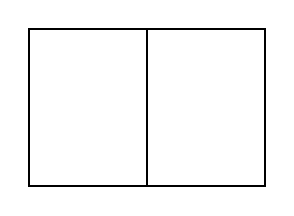
\begin{tikzpicture}
\draw [thick](0,0) rectangle (3,2);
\draw [thick](1.5,0) -- (1.5,2);
\end{tikzpicture}
\end{minipage}

\item A standard soda can is roughly cylindrical and holds $355$ cm$^3$ of liquid. What dimensions should the cylinder be to minimize the material needed to produce the can? Based on your dimensions, determine whether or not the standard can is produced to minimize the material costs.
\item Find the dimensions of a cylindrical can with a volume of $206$ in$^3$ that minimizes the surface area.

The ``\#10 can''is a standard sized can used by the restaurant industry that holds about $206$ in$^3$ with a diameter of $6 \frac{2}{16}$ in and height of $7$ in. Does it seem these dimensions where chosen with minimization in mind?

\item The strength $S$ of a wooden beam is directly proportional to its cross sectional  width $w$ and the square of its height $h$; that is, $S = kwh^2$ for some constant $k$. 

\noindent\begin{minipage}{\linewidth}
\centering
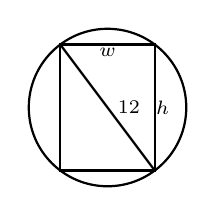
\begin{tikzpicture}
\draw [thick](0,0) circle (1cm);
\draw [thick](-.6,.8) -- node [pos=.5,right] {\scriptsize $12$} (.6,-.8);
\draw [thick](-.6,-.8) rectangle (.6,.8);
\draw (.7,0) node {\scriptsize $h$} (0,.7) node {\scriptsize $w$};
\end{tikzpicture}
\end{minipage}

Given a circular log with diameter of $12$ inches, what sized beam can be cut from the log with maximum strength?

\item A power line is to be run to an offshore facility in the manner described in Example~\ref{Ex:3.4.Eg3}. The offshore facility is $2$ miles at sea and $5$ miles along the shoreline from the power plant. It costs \$ $50,000$ per mile to lay a power line underground and \$ $80,000$ to run the line underwater. 

How much of the power line should be run underground to minimize the overall costs?
\item A power line is to be run to an offshore facility in the manner described in Example~\ref{Ex:3.4.Eg3}. The offshore facility is $5$ miles at sea and $2$ miles along the shoreline from the power plant. It costs $\$50,000$ per mile to lay a power line underground and $\$80,000$ to run the line underwater. 

How much of the power line should be run underground to minimize the overall costs?

\item A woman throws a stick into a lake for her dog to fetch; the stick is $20$ feet down the shore line and $15$ feet into the water from there. The dog may jump directly into the water and swim, or run along the shore line to get closer to the stick before swimming. The dog runs about $22$ ft/s and swims about $1.5$ ft/s. 

How far along the shore should the dog run to minimize the time it takes to get to the stick?

\item A woman throws a stick into a lake for her dog to fetch; the stick is $15$ feet down the shore line and $30$ feet into the water from there. The dog may jump directly into the water and swim, or run along the shore line to get closer to the stick before swimming. The dog runs about $22$ ft/s and swims about $1.5$ ft/s. 

How far along the shore should the dog run to minimize the time it takes to get to the stick? \textit{(Google ``calculus dog'' to learn more about a dog's ability to minimize times.)}

\item What are the dimensions of the rectangle with largest area that can be drawn inside the unit circle?

	\item A rectangular box with a square bottom and closed top is to be made from two materials.  The material for the side costs $\$1.50$ per square foot and the material for the bottom costs $\$3.00$ per square foot.  If you are willing to spend $\$15$ on the box, what is the largest volume it can contain?  Justify your answer completely using calculus.

\end{enumerate}

%------------------------------------------
% END OF EXERCISES ON FIRST PAGE
%------------------------------------------
\end{multicols*}
\end{adjustwidth*}

\clearpage

\begin{adjustwidth*}{}{-2.25in}
\setlength{\columnsep}{25pt}
\begin{multicols*}{2}\small

\begin{enumerate}[1),start=18]
	\item A farmer wants to start raising cows, horses, goats, and sheep, and desires to have a rectangular pasture for the animals to graze in.  However, no two different kinds of animals can graze together.  In order to minimize the amount of fencing she will need, she has decided to enclose a large rectangular area and then divide it into four equally sized pens, or grazing areas.  She has decided to purchase $7500$ ft of fencing.  What is the maximum possible area that each of the four pens will enclose?
	\item Two vertical towers of heights $60$ ft and $80$ ft stand on level ground, with their bases $100$ ft apart.  A cable that is stretched from the top of one pole to some point on the ground between the poles, and then to the top of the other pole.   What is the minimum possible length of cable required?  Justify your answer completely using calculus.
	\item A company is designing propane tanks that are cylindrical with hemispherical ends.   Assume that the company wants tanks that will hold $1000$ cubic feet of gas, and that the ends are more expensive to make, costing $\$5$ per square foot, while the cylindrical barrel between the ends costs $\$2$ per square foot.  Use calculus to determine the minimum cost to construct such a tank.
\end{enumerate}

%---------------------------------------------
% END OF EXERCISES ON SECOND PAGE
%---------------------------------------------
\end{multicols*}
\end{adjustwidth*}

\afterexercises 

\cleardoublepage